\documentclass{beamer}
\usepackage{moreverb} 
\usepackage{listings}
\usepackage{mflogo}
% imprimir
% \documentclass[handout]{beamer} 
% \usepackage{pgfpages}
% \pgfpagesuselayout{4 on 1}[a4paper,landscape,border shrink=5mm]

\mode<presentation> {
  \usetheme{Warsaw}
  \setbeamercovered{opaque}
}

\usebackgroundtemplate{
\includegraphics[width=\paperwidth]{format/libresoft-bg.png}}
\usepackage[spanish]{babel}
\usepackage[utf8]{inputenc}
\usepackage{graphics}
\usepackage{amssymb} % Simbolos matematicos

%% Metadatos del PDF.
\hypersetup{  
  pdftitle={Filtrado TCP/IP con software libre},
  pdfauthor={Miguel Vidal},
  pdfcreator={GSyC/Libresoft},
  pdfproducer=PDFLaTeX,
  pdfsubject={Master on Free Software},
}
%%

\defbeamertemplate*{footline}{shadow theme}
{%
  \leavevmode%
  \hbox{\begin{beamercolorbox}[wd=.5\paperwidth,ht=2.5ex,dp=1.125ex,leftskip=.1cm plus1fil,rightskip=.2cm]{author in head/foot}%

\includegraphics[scale=0.40]{format/cc-by-80x15.png} \hspace{0.05cm}
	Miguel Vidal / Jose Castro
  \end{beamercolorbox}%
  \begin{beamercolorbox}[wd=.5\paperwidth,ht=2.5ex,dp=1.125ex,leftskip=.3cm,rightskip=.3cm plus1fil]{title in head/foot}%
    \usebeamerfont{title in head/foot}\insertshorttitle%
    \hspace{2cm} \usebeamerfont{author in head/foot}\insertframenumber\,/\,\inserttotalframenumber\hfill
  \end{beamercolorbox}}%
  \vskip0pt%
}


\begin{document}

\title{Filtrado TCP/IP con software libre}
\subtitle{System Integration}
% \institute{\texttt{http://gsyc.urjc.es/\~{}mvidal} \\ Twitter: \texttt{@mvidallopez}}
\author{Miguel Vidal, Jose Castro} 
\date{\footnotesize{Master on Free Software \\ April 20th, 2012}}
\author{Miguel Vidal \hspace{1cm} Jose Castro \\
\hspace{0.5mm} {\tiny Twitter: @mvidallopez \hspace{1.1cm}Twitter: @jfcastroluis}
}


\frame{
\maketitle
\begin{center}

\includegraphics[width=6cm]{format/gsyc-urjc}
\end{center}
}

%% License slide
\begin{frame}
  \vspace{2cm}
  \begin{flushright}
    {\small \copyright{} 2011-2012 Miguel Vidal, Jose Castro} \\
%    \vspace{0.25cm}
    \medskip
    {\scriptsize This work is licensed under \\ a Creative Commons Attribution 3.0 License}
%    \vspace{0.10cm}
  \end{flushright}
  \begin{flushright}
    \href{http://creativecommons.org/licenses/by/3.0/es}{
\includegraphics[width=2cm]{format/cc-by.png}} \\
    {\tiny \url{http://creativecommons.org/licenses/by/3.0}}
  \end{flushright}
\end{frame}%%

\usebackgroundtemplate{}

\AtBeginSection[]
{
\begin{frame}<beamer>
\begin{center}
{\huge \insertsection}
\end{center}
\end{frame}
}


\AtBeginSubsection[]
{
  \begin{frame}<beamer>{Índice}
    \tableofcontents[currentsection,currentsubsection]
  \end{frame}
}

%%


%%%%%%%%%%%%%%%%%%%%%%%%%%%%%%%%%%%%%%%%%%%%%%%%%%%%%%%%%%%%%%%%%%%%%%%
\section{Cortafuegos y filtrado TCP/IP}
%%%%%%%%%%%%%%%%%%%%%%%%%%%%%%%%%%%%%%%%%%%%%%%%%%%%%%%%%%%%%%%%%%%%%%%

%%%%%%%%%%%%%%%%%%%%%%%%%%%%%%%%%%%%%%%%%%%%%%%%%%%%%%%%%%%%%%%%%%%%%%%

\begin{frame}
\frametitle{¿Qué es un cortafuegos? (1)}

\begin{itemize}
\item FW (Firewall): término usado para referirse a cosas muy dispares en los últimos años.
\item Se llama lo mismo al FW casero que te colocan en tu línea ADSL o al que le cuesta miles de dólares en una empresa.
\item ¿Qué diferencias hay?

	\begin{itemize}
	\item Funcionalidades que ofrece.
	\item Hardware en el que corre.
	\item Robustez y fiabilidad de su software.
	\end{itemize}

\end{itemize}
\end{frame}

%%%%%%%%%%%%%%%%%%%%%%%%%%%%%%%%%%%%%%%%%%%%%%%%%%%%%%%%%%%%%%%%%%%%%%%

\begin{frame}
\frametitle{¿Qué es un cortafuegos? (2)}

\begin{itemize}
\item Software que funciona como punto de regulación entre un grupo de redes (normalmente una red privada y una red pública).
\item Son ubicuos: herramienta básica para la seguridad de redes.
\item Todo el tráfico de red entre las redes involucradas se encamina a través del cortafuegos.
\item En grandes corporaciones puede haber cortafuegos dentro de la red corporativa para aislar las zonas importantes de la organización.
\item Crear cortafuegos es un arte: exige comprender muy bien la tecnología de red subyacente.
\end{itemize}

\end{frame}


%%%%%%%%%%%%%%%%%%%%%%%%%%%%%%%%%%%%%%%%%%%%%%%%%%%%%%%%%%%%%%%%%%%%%%%

\begin{frame}
\frametitle{¿Qué es un cortafuegos? (y 3)}

\begin{itemize}
\item Un cortafuegos se configura mediante un conjunto de reglas que determina qué tráfico puede pasar y cuál será bloqueado (con respuesta) o desechado (sin respuesta).
\item Los cortafuegos pueden situarse de formas distintas: 
	\begin{itemize}
	\item La forma más simple (e insegura) es un solo equipo que además proporciona otros servicios.
	\item La forma más sofisticada son las DMZ (o red perimetral), que puede involucrar a varios equipos cortafuegos. 
	\end{itemize}
\end{itemize}

\end{frame}

%%%%%%%%%%%%%%%%%%%%%%%%%%%%%%%%%%%%%%%%%%%%%%%%%%%%%%%%%%%%%%%%%%%%%%%

\begin{frame}
\frametitle{Diseño de cortafuegos con un solo firewall}

\begin{figure}[h]

\begin{center}
  \centering
  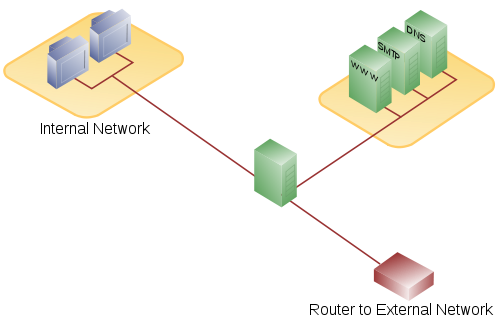
\includegraphics[height=2.7in]{figs/500px-DMZ_network_diagram_1_firewall.png}
  %\caption{Diseño sencillo de UN FW. \textit{Fuente:} Wikipedia.}
\end{center}
\end{figure}

\end{frame}

%%%%%%%%%%%%%%%%%%%%%%%%%%%%%%%%%%%%%%%%%%%%%%%%%%%%%%%%%%%%%%%%%%%%%%%

\begin{frame}
\frametitle{Diseño de cortafuegos con 2 firewalls (DMZ)}

\begin{figure}[h]

\begin{center}
  \centering
  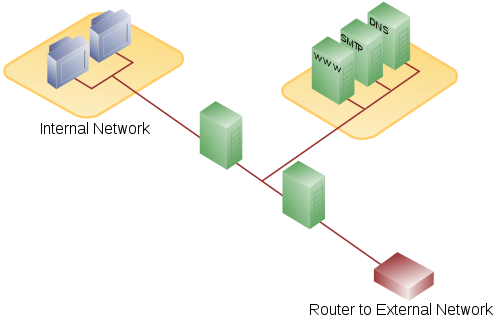
\includegraphics[height=2.7in]{figs/500px-DMZ_network_diagram_2_firewall.png}
%  \caption{2 firewalls. \textit{Fuente:} Wikipedia.}
\end{center}
\end{figure}

\end{frame}


%%%%%%%%%%%%%%%%%%%%%%%%%%%%%%%%%%%%%%%%%%%%%%%%%%%%%%%%%%%%%%%%%%%%%%%

\begin{frame}
\frametitle{Tipos de procesado de paquetes}

\begin{itemize}
\item \alert{Filtrado:} decidir en distintos momentos del flujo si un paquete pasa o es bloqueado.
\item \alert{Modificación:} modificación mientras se mueve el flujo de paquetes
\item \alert{Traducción (NAT)}: permite redirigir el tráfico de forma transparente mediante la modificación de la fuente, el destino o los puertos.
\end{itemize}

\end{frame}

%%%%%%%%%%%%%%%%%%%%%%%%%%%%%%%%%%%%%%%%%%%%%%%%%%%%%%%%%%%%%%%%%%%%%%%

\begin{frame}
\frametitle{¿Qué es el filtrado de IP?}

El filtrado IP consiste en decidir qué paquetes se procesarán y cuáles serán rechazados. Algunos criterios posibles para filtrar:

\begin{itemize}
\item Tipo de protocolo: TCP, UDP, ICMP, etc.
\item Número de puerto (para TCP/UDP)
\item Tipo de paquete: SYN/ACK, datos, petición de eco ICMP...
\item Origen del paquete
\item Destino del paquete
\end{itemize}

Los conjuntos de reglas (\textit{rulesets}) se componen mediante combinación de algunos de estos criterios.

\end{frame}

%%%%%%%%%%%%%%%%%%%%%%%%%%%%%%%%%%%%%%%%%%%%%%%%%%%%%%%%%%%%%%%%%%%%%%%

\begin{frame}
\frametitle{¿Qué es el filtrado de IP?}

\begin{itemize}
\item El filtrado IP es una utilidad de capa de red (layer-3).
\item No conoce nada de las aplicaciones que usan las conexiones de red.
\item Por ejemplo, si filtramos por puerto, ese mismo servicio podría ejecutarse en otro puerto y el firewall no lo impediría.
\item Para solucionar esto, se usan \alert{servidores proxy}, que gestionan la conexión y sí comprenden el servicio.
\end{itemize}

\end{frame}

%%%%%%%%%%%%%%%%%%%%%%%%%%%%%%%%%%%%%%%%%%%%%%%%%%%%%%%%%%%%%%%%%%%%%%%

\begin{frame}
\frametitle{Conceptos básicos}

\begin{itemize}
\item \textit{default accept} versus \textit{default deny}.
\item Inspección de paquetes: \alert{Stateful} vs \alert{stateless}  
\item En los FW de primera generación no habia estado, lo que facilitaba el \textit{spoofing}.
\item La inspección de estado guarda registros de todas las conexiones de red que pasan por el cortafuegos.
\item Establecimiento de la comunicación TCP en tres pasos (\textit{Three-way handshake}):

\begin{itemize}
	\item \alert{SYN packet}: solicitud de sincronización
	\item \alert{SYN+ACK packet}: sincronización y acuse de recibo del servidor
	\item \alert{ACK packet}: acuse de recibo (\textit{acknowledgment}) del cliente.
\end{itemize}

\end{itemize}

\end{frame}


%%%%%%%%%%%%%%%%%%%%%%%%%%%%%%%%%%%%%%%%%%%%%%%%%%%%%%%%%%%%%%%%%%%%%%%

\begin{frame}
\frametitle{Filtrado de paquetes}

\begin{itemize}
\item Un firewall avanzado puede hacer más cosas además de bloquear. 
\item Realiza otras funcionalidades importantes: enmascaramiento, NAT, auditorías, gestión de ancho de banda, balanceo de carga, filtrado por criterios específicos, redundancia...
\end{itemize}

\end{frame}

%%%%%%%%%%%%%%%%%%%%%%%%%%%%%%%%%%%%%%%%%%%%%%%%%%%%%%%%%%%%%%%%%%%%%%%

\begin{frame}
\frametitle{Herramientas libres para filtrado de paquetes}

\begin{itemize}
\item \alert{\texttt{iptables}}: Linux
\item \alert{\texttt{ipfilter}}: *Solaris, illumos, FreeBSD, NetBSD, Linux, HP-UX, IRIX
\item \alert{\texttt{PF (Packet Filter)}}: OpenBSD (nativo), FreeBSD, NetBSD, DragonFly.
\end{itemize}

Comparativa: \url{http://en.wikipedia.org/wiki/Comparison_of_firewalls}

\end{frame}

%%%%%%%%%%%%%%%%%%%%%%%%%%%%%%%%%%%%%%%%%%%%%%%%%%%%%%%%%%%%%%%%%%%%%%%

\begin{frame}
\frametitle{¿Son seguros?}

\begin{itemize}
\item Muy habitual usar sistemas dedicados como Cisco (privativo)
\item Sistemas operativos de propósito general son más vulnerables.
\item Bien configurados, pueden ser igual de seguros, y más baratos.
\item Hay soluciones profesionales de software libre dedicadas a \textit{firewalling} (como \alert{pfSense}, basada en OpenBSD PF).
\item La seguridad es una estrategia multicapa, no solo un firewall: cada equipo debe ser individualmente parcheado, actualizado y monitorizado.
\end{itemize}

Comparativa: \url{http://en.wikipedia.org/wiki/Comparison_of_firewalls}

\end{frame}


%%%%%%%%%%%%%%%%%%%%%%%%%%%%%%%%%%%%%%%%%%%%%%%%%%%%%%%%%%%%%%%%%%%%%%%
\section{Firewall con Linux: Netfilter/iptables}
%%%%%%%%%%%%%%%%%%%%%%%%%%%%%%%%%%%%%%%%%%%%%%%%%%%%%%%%%%%%%%%%%%%%%%%

%%%%%%%%%%%%%%%%%%%%%%%%%%%%%%%%%%%%%%%%%%%%%%%%%%%%%%%%%%%%%%%%%%%%%%%

\begin{frame}
\frametitle{Implementaciones de filtrado en Linux}

\begin{itemize}
\item \alert{1ª generación:} Port de ipfw de Unix BSD a Linux 1.1 (Alan Cox)
\item \alert{2ª generación:} Jos Vos y otros añaden ipfwadm a Linux 1.1
\item \alert{3ª generación:} Rusty Russell y Michael Neuling hacen cambios importantes a ipfw, ipchains se publica en Linux 2.2
\item \alert{4ª generación:} Rusty (junto a otros) implementa una infrastructura modular para el kernel Linux 2.4 a la que denomina \alert{Netfilter}.
\item \alert{iptables} son las herramientas CLI ejecutadas en espacio de usuario para manejar NetFilter.
\end{itemize}

\end{frame}

%%%%%%%%%%%%%%%%%%%%%%%%%%%%%%%%%%%%%%%%%%%%%%%%%%%%%%%%%%%%%%%%%%%%%%%

\begin{frame}
\frametitle{Fundamentos de Netfilter/iptables}

\begin{itemize}
\item Es la herramienta estándar de todas las distribuciones Linux modernas.
\item Se basa en cadenas (``\alert{chains}'') de reglas aplicadas a los paquetes de red.
\item Los conjuntos de cadenas (reglas) se almacenan en ``tablas''(\alert{tables}).
\end{itemize}

\end{frame}


%%%%%%%%%%%%%%%%%%%%%%%%%%%%%%%%%%%%%%%%%%%%%%%%%%%%%%%%%%%%%%%%%%%%%%%

\begin{frame}
\frametitle{Tablas}

iptables dispone de tres tablas predefinidas para almacenar las reglas:

	\begin{enumerate}
	\item \textsc{filter}: es la tabla por defecto.
	\item \textsc{nat}: contiene las reglas que controlan la traducción de direcciones (NAT).
	\item \textsc{mangle}: modifica el contenido de paquetes.
	\end{enumerate}

\end{frame}

%%%%%%%%%%%%%%%%%%%%%%%%%%%%%%%%%%%%%%%%%%%%%%%%%%%%%%%%%%%%%%%%%%%%%%%
\begin{frame}
\frametitle{Cadenas de la tabla \textsc{filter}}

La tabla \alert{filter} contiene tres cadenas de reglas estándar: 
	\begin{itemize}
	\item \textsc{input}: se aplica al tráfico que tiene como destino el host local.
	\item \textsc{output}: se aplica a paquetes originados en el host local redirigidos al exterior.
	\item \textsc{forward}: se aplica a los paquetes enrutados que no tienen destino local.
	\end{itemize}

\end{frame}

%%%%%%%%%%%%%%%%%%%%%%%%%%%%%%%%%%%%%%%%%%%%%%%%%%%%%%%%%%%%%%%%%%%%%%%
\begin{frame}
\frametitle{Cadenas de la tabla \textsc{nat}}

La tabla \alert{nat} contiene las siguientes cadenas de reglas estándar: 
	\begin{itemize}
        \item \textsc{prerouting} se aplica a los paquetes antes de ser enrutados
        \item \textsc{postrouting} se aplica a los paquetes cuando ya han sido enrutados
	\item \textsc{output}: se aplica a paquetes originados en el host local redirigidos al exterior
	\end{itemize}

\end{frame}

%%%%%%%%%%%%%%%%%%%%%%%%%%%%%%%%%%%%%%%%%%%%%%%%%%%%%%%%%%%%%%%%%%%%%%%
\begin{frame}
\frametitle{Cadenas de la tabla \textsc{mangle}}

La tabla \alert{mangle} contiene las siguientes cadenas de reglas estándar: 
	\begin{itemize}
	\item \textsc{input}: se aplica al tráfico dirigido al host local
	\item \textsc{output}: se aplica al tráfico originado en el host local
        \item \textsc{forward}
        \item \textsc{prerouting}: 
        \item \textsc{postrouting}
	\end{itemize}

\end{frame}


%%%%%%%%%%%%%%%%%%%%%%%%%%%%%%%%%%%%%%%%%%%%%%%%%%%%%%%%%%%%%%%%%%%%%%%

\begin{frame}
\frametitle{Rule targets}

\begin{itemize}
\item Cada regla que compone una cadena especifica una acción o \alert{target}.
\item Las reglas se procesan en orden hasta que se cumple una condición.
\item Reglas disponibles en la tabla filter:
	\begin{itemize}
	\item \textsc{accept}: permite al paquete seguir su camino
	\item \textsc{drop} (descarte silencioso) 
	\item \textsc{reject} (mensaje icmp)
	\item \textsc{log} (traza el paquete), \textsc{mirror}...
	\end{itemize}
\end{itemize}

\end{frame}

%%%%%%%%%%%%%%%%%%%%%%%%%%%%%%%%%%%%%%%%%%%%%%%%%%%%%%%%%%%%%%%%%%%%%%%

\begin{frame}
\frametitle{Configuración}


\begin{block}{Activar IP forwarding}
\# echo 1 $>$ /proc/sys/net/ipv4/ip\_forward
\end{block}

\begin{block}{Activar IP forwarding de forma permanente}
en /etc/sysctl.conf: \\
net.ipv4.ip\_forward $=$ 1 \\
\# sysctl -p /etc/sysctl.conf
\end{block}

\begin{itemize}
\item Asegurarse de que los módulos del kernel están disponibles
\end{itemize}

\end{frame}


%%%%%%%%%%%%%%%%%%%%%%%%%%%%%%%%%%%%%%%%%%%%%%%%%%%%%%%%%%%%%%%%%%%%%%%

\begin{frame}
\frametitle{Funcionamiento de iptables}

\begin{block}{Forma de los comandos de iptables}
\alert{iptables -F chain-name} \# -F limpia reglas anteriores \\
\alert{iptables -P chain-name target} \# -P fija una política (target) por defecto \\
\alert{iptables -A chain-name -i interface -j target} \# -A añade nueva regla \\
\alert{iptables -D}  \# borra una regla \\
\end{block}

Estos comandos suelen incluirse en un script de inicio rc.

\begin{block}{Ver reglas cargadas}
\# iptables -L
\end{block}

\end{frame}


%%%%%%%%%%%%%%%%%%%%%%%%%%%%%%%%%%%%%%%%%%%%%%%%%%%%%%%%%%%%%%%%%%%%%%%

\begin{frame}
\frametitle{Opciones más comunes}


\begin{itemize}
\item \texttt{-p}: define protocolos (TCP, UDP, etc.).
\item \texttt{-s}: define tráfico de origen
\item \texttt{-d}: define tráfico de destino
\item \texttt{$--$source-port}: define el puerto desde el que se origina la conexión
\item \texttt{$--$destination-port}: define el puerto hacia el que se dirige la conexión
\item \texttt{-t}: tabla a utilizar (nat, filter, mangle o raw)
\item \texttt{-o}: define una interfaz para tráfico saliente
\end{itemize}

\end{frame}

%%%%%%%%%%%%%%%%%%%%%%%%%%%%%%%%%%%%%%%%%%%%%%%%%%%%%%%%%%%%%%%%%%%%%%%

\begin{frame}[fragile]
\frametitle{Cómo iptables procesa los paquetes}

  \begin{center}
    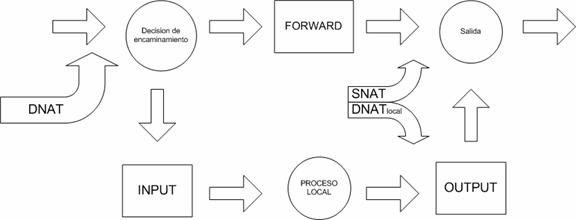
\includegraphics[width=9cm]{figs/iptables-flow.jpg}
  \end{center}

\end{frame}

%%%%%%%%%%%%%%%%%%%%%%%%%%%%%%%%%%%%%%%%%%%%%%%%%%%%%%%%%%%%%%%%%%%%%%%

\begin{frame}[fragile]
\frametitle{Cómo iptables procesa los paquetes}

\begin{verbatim}
PACKET IN
    |
PREROUTING--[routing]-->--FORWARD-->--POSTROUTING-->--OUT
 - nat (dst)   |           - filter      - nat (src)
               |                            |
               |                            |
              INPUT                       OUTPUT
              - filter                    - nat (dst)
               |                          - filter
               |                            |
               `----->-----[app]----->------'
\end{verbatim}

\end{frame}


%%%%%%%%%%%%%%%%%%%%%%%%%%%%%%%%%%%%%%%%%%%%%%%%%%%%%%%%%%%%%%%%%%%%%%%

\begin{frame}
\frametitle{Limpieza de reglas}

\begin{block}{Limpieza (flush) de reglas}
iptables -F INPUT \\
iptables -F FORWARD \\
iptables -F OUTPUT \\
iptables -F -t nat
\end{block}

\end{frame}


%%%%%%%%%%%%%%%%%%%%%%%%%%%%%%%%%%%%%%%%%%%%%%%%%%%%%%%%%%%%%%%%%%%%%%%

\begin{frame}
\frametitle{Políticas por defecto}

\begin{block}{Policies por defecto}
iptables -F 
iptables -P INPUT DROP \\
iptables -P FORWARD DROP  \\
\end{block}

\end{frame}

%%%%%%%%%%%%%%%%%%%%%%%%%%%%%%%%%%%%%%%%%%%%%%%%%%%%%%%%%%%%%%%%%%%%%%%

\begin{frame}
\frametitle{Aplicar algunas reglas}

\begin{block}{Aplicar algunas reglas}
iptables -A FORWARD -i eth0 -p ANY -j ACCEPT  \\
iptables -A FORWARD -d 10.1.1.2 -p tcp -dport 80 -j ACCEPT \\
iptables -A FORWARD -d 10.1.1.2 -p tcp -dport 22 -j ACCEPT   \\
\end{block}

Los comandos suelen incluirse en un script de inicio rc (\texttt{/etc/network/if-pre-up.d} y \texttt{/etc/network/if-post-down.d} en Debian/Ubuntu)

\end{frame}

%%%%%%%%%%%%%%%%%%%%%%%%%%%%%%%%%%%%%%%%%%%%%%%%%%%%%%%%%%%%%%%%%%%%%%%

\begin{frame}
\frametitle{Mantener estado}

Permite tráfico de entrada con las conexiones que ha iniciado nuestro host:

\begin{block}{Stateful packet filtering}
iptables -A FORWARD -i eth0 -p ANY -j ACCEPT  \\
iptables -A FORWARD -m state $--$state ESTABLISHED,RELATED -j ACCEPT \\
\end{block}

\end{frame}



%%%%%%%%%%%%%%%%%%%%%%%%%%%%%%%%%%%%%%%%%%%%%%%%%%%%%%%%%%%%%%%%%%%%%%%

\begin{frame}[fragile]
\frametitle{Reenvío de puertos con iptables}

  \begin{center}
    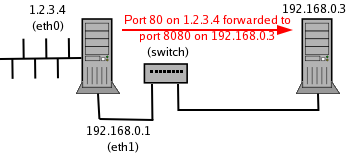
\includegraphics[width=9cm]{figs/port-forwarding.png}
  \end{center}

\end{frame}


%%%%%%%%%%%%%%%%%%%%%%%%%%%%%%%%%%%%%%%%%%%%%%%%%%%%%%%%%%%%%%%%%%%%%%%


\begin{frame}[fragile]
\frametitle{Reenvío de puertos con iptables}

\begin{verbatim}
Internet---------[router/firewall]-------------LAN 
0.0.0.0/0      1.2.3.4    192.168.0.1    192.168.0.0/24
\end{verbatim}

\begin{block}{Reglas para port forwarding}
\small
\# iptables -A PREROUTING -t nat -i eth0 -p tcp $--$dport 80 -j DNAT $--$to 192.168.0.3:8080 \\
\# iptables -A FORWARD -p tcp -d 192.168.0.3 $--$dport 8080 -j ACCEPT
\end{block}

Nota: la segunda regla debe aplicarse si negamos todas las conexiones entrantes por defecto. 

\end{frame}



\begin{frame}[fragile]
\frametitle{Reenvío de puertos con iptables}

\begin{verbatim}
Internet---------[router/firewall]-------------LAN 
0.0.0.0/0      1.2.3.4    192.168.0.1    192.168.0.0/24
\end{verbatim}

\begin{block}{Reglas para port forwarding}
\small
\# iptables -A PREROUTING -t nat -i eth0 -p tcp $--$dport 80 -j DNAT $--$to 192.168.0.3:8080 \\
\# iptables -A FORWARD -p tcp -d 192.168.0.3 $--$dport 8080 -j ACCEPT
\end{block}

\end{frame}


%%%%%%%%%%%%%%%%%%%%%%%%%%%%%%%%%%%%%%%%%%%%%%%%%%%%%%%%%%%%%%%%%%%%%%%

\begin{frame}
\frametitle{Referencias}

\begin{itemize}
\item Tony Bautts, Terry Dawson y Gregor N. Purdy. \textit{Linux Network Administrator's Guide}, O'Reilly (existe edición en español).
\item Peter N.M. Hansteen, \textit{The Book of PF}, 2nd Edition, No Starch, 2011.
\end{itemize}

\end{frame}


%%%%%%%%%%%%%%%%%%%%%%%%%%%%%%%%%%%%%%%%%%%%%%%%%%%%%%%%%%%%%%%%%%%%%%


\frame{
\maketitle
\begin{center}

\includegraphics[width=6cm]{format/gsyc-urjc}
\end{center}
}

\end{document}

